\documentclass[12pt]{article}


% Template-specific packages
\usepackage[utf8]{inputenc} % Required for inputting international characters
\usepackage[T1]{fontenc} % Output font encoding for international characters

\usepackage{mathpazo} % Use the Palatino font

\usepackage{booktabs} % Required for better horizontal rules in tables

\usepackage{listings} % Required for insertion of code

\usepackage{enumerate} % To modify the enumerate environment


\title{Parallel Homework \#1}
\author{liukanglai} 
\date{\today}
\usepackage{graphicx}
\graphicspath{{./}}

\usepackage{listings}
\usepackage{xcolor}
\lstset{
    numbers=left,
    numberstyle= \tiny,
    keywordstyle= \color{ blue!70},
    commentstyle= \color{red!50!green!50!blue!50},
    frame=shadowbox, % 阴影效果
    rulesepcolor= \color{ red!20!green!20!blue!20} ,
    escapeinside=``, % 英文分号中可写入中文
    xleftmargin=2em,xrightmargin=2em, aboveskip=1em,
    framexleftmargin=2em
}


\begin{document}

\maketitle

\newpage

\begin{figure}[h]
\centering
\caption{Here is the hardware's information}
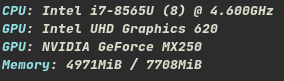
\includegraphics[scale=0.5]{HardwareInfo}
\caption{Here is the cupcores' information}
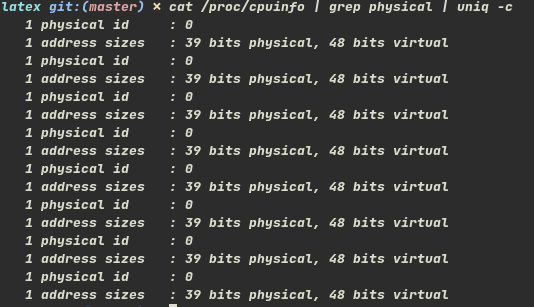
\includegraphics[scale=0.5]{cup_cores}
\caption{Here is the test runing}
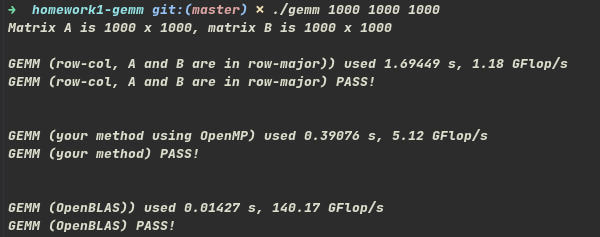
\includegraphics[scale=0.5]{testrunning}
\end{figure}


To get the following data is annoying, for there are many operations to do.

And to write a script will reduce a lot of work.

\newpage
Such as: 

\begin{lstlisting}
./gemm 100 100 100 > 1.txt
./gemm 200 200 200 >> 1.txt
./gemm 300 300 300 >> 1.txt
./gemm 400 400 400 >> 1.txt
./gemm 500 500 500 >> 1.txt
./gemm 600 600 600 >> 1.txt
./gemm 700 700 700 >> 1.txt
./gemm 800 800 800 >> 1.txt
./gemm 900 900 900 >> 1.txt
./gemm 1000 1000 1000 >> 1.txt
./gemm 1100 1100 1100 >> 1.txt
./gemm 1200 1200 1200 >> 1.txt
./gemm 1300 1300 1300 >> 1.txt
./gemm 1400 1400 1400 >> 1.txt
./gemm 1500 1500 1500 >> 1.txt
./gemm 1600 1600 1600 >> 1.txt
./gemm 1700 1700 1700 >> 1.txt
./gemm 1800 1800 1800 >> 1.txt
./gemm 1900 1900 1900 >> 1.txt
./gemm 2000 2000 2000 >> 1.txt
\end{lstlisting}

save it as 1.sh, then ./1.sh(you may need chmod +x 1.sh)


To get the data for painting, I find a good command:
\begin{lstlisting}
echo $(grep -Eo '[0-9\.]+' myfile.txt) >output.txt
\end{lstlisting}


\newpage
\section{the original serial code}

GEMM (row-col, A and B are in row-major)) used 0.00102 s, 1.96 GFlop/s

GEMM (your method)) used 0.00057 s, 3.52 GFlop/s

GEMM (row-col, A and B are in row-major)) used 0.00880 s, 1.82 GFlop/s

GEMM (your method)) used 0.00412 s, 3.89 GFlop/s

GEMM (row-col, A and B are in row-major)) used 0.02998 s, 1.80 GFlop/s

GEMM (your method)) used 0.01348 s, 4.00 GFlop/s

GEMM (row-col, A and B are in row-major)) used 0.06944 s, 1.84 GFlop/s

GEMM (your method)) used 0.01855 s, 6.90 GFlop/s

GEMM (row-col, A and B are in row-major)) used 0.11889 s, 2.10 GFlop/s

GEMM (your method)) used 0.03502 s, 7.14 GFlop/s

GEMM (row-col, A and B are in row-major)) used 0.20949 s, 2.06 GFlop/s

GEMM (your method)) used 0.06048 s, 7.14 GFlop/s

GEMM (row-col, A and B are in row-major)) used 0.33802 s, 2.03 GFlop/s

GEMM (your method)) used 0.09937 s, 6.90 GFlop/s

GEMM (row-col, A and B are in row-major)) used 0.56159 s, 1.82 GFlop/s

GEMM (your method)) used 0.14351 s, 7.14 GFlop/s

GEMM (row-col, A and B are in row-major)) used 0.82811 s, 1.76 GFlop/s

GEMM (your method)) used 0.23620 s, 6.17 GFlop/s

GEMM (row-col, A and B are in row-major)) used 1.72386 s, 1.16 GFlop/s

GEMM (your method)) used 0.38879 s, 5.14 GFlop/s

GEMM (row-col, A and B are in row-major)) used 2.22392 s, 1.20 GFlop/s

GEMM (your method)) used 0.53795 s, 4.95 GFlop/s

GEMM (row-col, A and B are in row-major)) used 3.24518 s, 1.06 GFlop/s

GEMM (your method)) used 0.76877 s, 4.50 GFlop/s

GEMM (row-col, A and B are in row-major)) used 5.12792 s, 0.86 GFlop/s

GEMM (your method)) used 1.05956 s, 4.15 GFlop/s

GEMM (row-col, A and B are in row-major)) used 5.56816 s, 0.99 GFlop/s

GEMM (your method)) used 1.36282 s, 4.03 GFlop/s

GEMM (row-col, A and B are in row-major)) used 8.89214 s, 0.76 GFlop/s

GEMM (your method)) used 2.07073 s, 3.26 GFlop/s

GEMM (row-col, A and B are in row-major)) used 13.07524 s, 0.63 GFlop/s

GEMM (your method)) used 2.29913 s, 3.56 GFlop/s

GEMM (row-col, A and B are in row-major)) used 17.75225 s, 0.55 GFlop/s

GEMM (your method)) used 2.44229 s, 4.02 GFlop/s

GEMM (row-col, A and B are in row-major)) used 20.95926 s, 0.56 GFlop/s

GEMM (your method)) used 2.89090 s, 4.03 GFlop/s

GEMM (row-col, A and B are in row-major)) used 28.11750 s, 0.49 GFlop/s

GEMM (your method)) used 3.42984 s, 4.00 GFlop/s

GEMM (row-col, A and B are in row-major)) used 31.26064 s, 0.51 GFlop/s

GEMM (your method)) used 4.86276 s, 3.29 GFlop/s

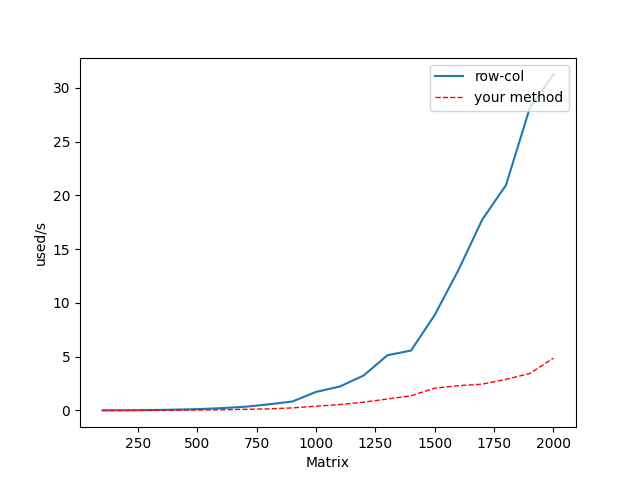
\includegraphics[scale=0.5]{1s}
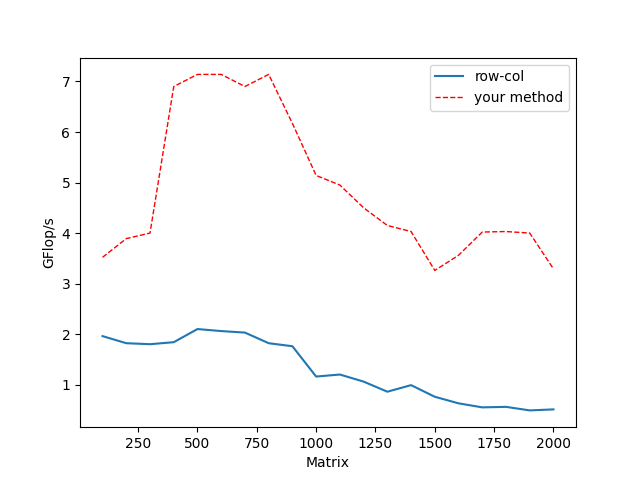
\includegraphics[scale=0.5]{1g}

\section{several kinds of serial codes in exchange order}

\subsection{i, ki, j}

used 0.00056 s, 3.57 GFlop/s

used 0.00412 s, 3.88 GFlop/s

used 0.01338 s, 4.03 GFlop/s

used 0.03295 s, 3.88 GFlop/s

used 0.03635 s, 6.88 GFlop/s

used 0.06897 s, 6.26 GFlop/s

used 0.09563 s, 7.17 GFlop/s

used 0.15294 s, 6.70 GFlop/s

used 0.23971 s, 6.08 GFlop/s

used 0.39362 s, 5.08 GFlop/s

used 0.57278 s, 4.65 GFlop/s

used 0.74118 s, 4.66 GFlop/s

used 1.01079 s, 4.35 GFlop/s

used 1.38078 s, 3.97 GFlop/s

used 1.69293 s, 3.99 GFlop/s

used 2.00908 s, 4.08 GFlop/s

used 2.46988 s, 3.98 GFlop/s

used 3.07154 s, 3.80 GFlop/s

used 3.60899 s, 3.80 GFlop/s

used 4.24184 s, 3.77 GFlop/s

\subsection{i, j, ki}

used 0.00133 s, 1.51 GFlop/s

used 0.01035 s, 1.55 GFlop/s

used 0.03485 s, 1.55 GFlop/s

used 0.06523 s, 1.96 GFlop/s

used 0.12682 s, 1.97 GFlop/s

used 0.21508 s, 2.01 GFlop/s

used 0.35496 s, 1.93 GFlop/s

used 0.61810 s, 1.66 GFlop/s

used 0.94968 s, 1.54 GFlop/s

used 1.77247 s, 1.13 GFlop/s

used 2.44696 s, 1.09 GFlop/s

used 3.23357 s, 1.07 GFlop/s

used 5.82691 s, 0.75 GFlop/s

used 6.08800 s, 0.90 GFlop/s

used 8.87992 s, 0.76 GFlop/s

used 13.04372 s, 0.63 GFlop/s

used 17.98408 s, 0.55 GFlop/s

used 22.23343 s, 0.52 GFlop/s

used 29.17877 s, 0.47 GFlop/s

used 30.89221 s, 0.52 GFlop/s

\subsection{ki, i, j}

used 0.00053 s, 3.78 GFlop/s

used 0.00406 s, 3.94 GFlop/s

used 0.03598 s, 1.50 GFlop/s

used 0.02632 s, 4.86 GFlop/s

used 0.03591 s, 6.96 GFlop/s

used 0.06295 s, 6.86 GFlop/s

used 0.10332 s, 6.64 GFlop/s

used 0.18250 s, 5.61 GFlop/s

used 0.26754 s, 5.45 GFlop/s

used 0.43052 s, 4.65 GFlop/s

used 0.67797 s, 3.93 GFlop/s

used 0.97233 s, 3.55 GFlop/s

used 1.36233 s, 3.23 GFlop/s

used 2.00249 s, 2.74 GFlop/s

used 2.40162 s, 2.81 GFlop/s

used 2.64902 s, 3.09 GFlop/s

used 4.22108 s, 2.33 GFlop/s

used 4.12343 s, 2.83 GFlop/s

used 6.65517 s, 2.06 GFlop/s

used 5.77122 s, 2.77 GFlop/s

\subsection{ki, j, i}

used 0.00098 s, 2.04 GFlop/s

used 0.00928 s, 1.72 GFlop/s

used 0.03800 s, 1.42 GFlop/s

used 0.08881 s, 1.44 GFlop/s

used 0.13573 s, 1.84 GFlop/s

used 0.24446 s, 1.77 GFlop/s

used 0.55681 s, 1.23 GFlop/s

used 2.19454 s, 0.47 GFlop/s

used 4.55634 s, 0.32 GFlop/s

used 6.51371 s, 0.31 GFlop/s

used 9.83481 s, 0.27 GFlop/s

used 14.24950 s, 0.24 GFlop/s

used 17.21507 s, 0.26 GFlop/s

used 22.67421 s, 0.24 GFlop/s

used 28.51237 s, 0.24 GFlop/s

used 34.44606 s, 0.24 GFlop/s

used 42.11570 s, 0.23 GFlop/s

used 51.29658 s, 0.23 GFlop/s

used 61.06770 s, 0.22 GFlop/s

used 72.93995 s, 0.22 GFlop/s

\subsection{j, ki, i}

used 0.00098 s, 2.03 GFlop/s

used 0.00932 s, 1.72 GFlop/s

used 0.03746 s, 1.44 GFlop/s

used 0.08922 s, 1.43 GFlop/s

used 0.13562 s, 1.84 GFlop/s

used 0.26870 s, 1.61 GFlop/s

used 0.53022 s, 1.29 GFlop/s

used 2.11891 s, 0.48 GFlop/s

used 4.94585 s, 0.29 GFlop/s

used 6.61430 s, 0.30 GFlop/s

used 10.81202 s, 0.25 GFlop/s

used 13.89475 s, 0.25 GFlop/s

used 20.35850 s, 0.22 GFlop/s

used 23.19168 s, 0.24 GFlop/s

used 32.24834 s, 0.21 GFlop/s

used 40.34462 s, 0.20 GFlop/s

used 47.24516 s, 0.21 GFlop/s

used 53.48966 s, 0.22 GFlop/s

used 67.74452 s, 0.20 GFlop/s

used 74.35895 s, 0.22 GFlop/s

\subsection{j, i, ki}

used 0.00133 s, 1.50 GFlop/s

used 0.01118 s, 1.43 GFlop/s

used 0.02688 s, 2.01 GFlop/s

used 0.07242 s, 1.77 GFlop/s

used 0.12366 s, 2.02 GFlop/s

used 0.21535 s, 2.01 GFlop/s

used 0.34364 s, 2.00 GFlop/s

used 0.63364 s, 1.62 GFlop/s

used 0.78422 s, 1.86 GFlop/s

used 1.57273 s, 1.27 GFlop/s

used 1.55374 s, 1.71 GFlop/s

used 2.28916 s, 1.51 GFlop/s

used 3.14497 s, 1.40 GFlop/s

used 3.43000 s, 1.60 GFlop/s

used 5.41349 s, 1.25 GFlop/s

used 10.87437 s, 0.75 GFlop/s

used 13.99641 s, 0.70 GFlop/s

used 18.79972 s, 0.62 GFlop/s

used 25.27928 s, 0.54 GFlop/s

used 28.75452 s, 0.56 GFlop/s

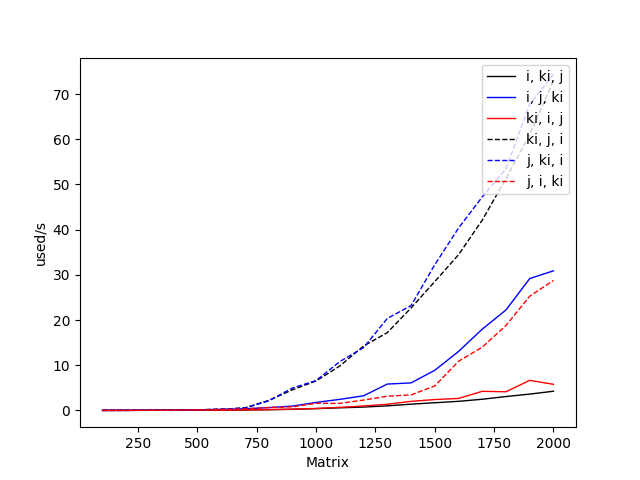
\includegraphics[scale=0.5]{2s}
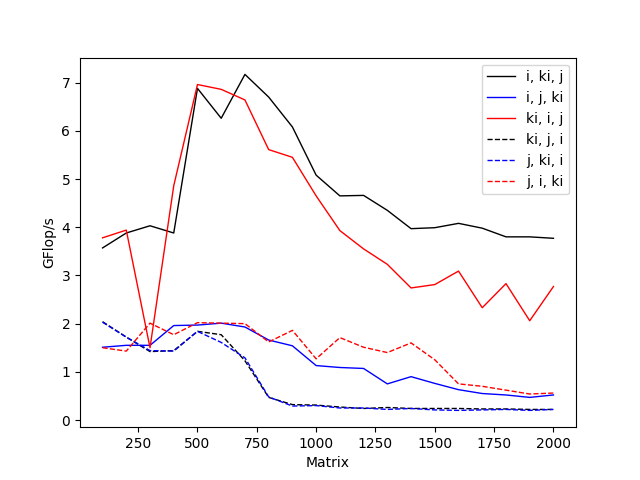
\includegraphics[scale=0.5]{2g}

\section{The parallel code of adding OpenMP instruction statements on different for loops}
\subsection{On the outermost layer}

GEMM (your method using OpenMP) used 0.02339 s, 0.09 GFlop/s

GEMM (your method using OpenMP) used 0.04390 s, 0.36 GFlop/s

GEMM (your method using OpenMP) used 0.02608 s, 2.07 GFlop/s

GEMM (your method using OpenMP) used 0.02916 s, 4.39 GFlop/s

GEMM (your method using OpenMP) used 0.00826 s, 30.27 GFlop/s

GEMM (your method using OpenMP) used 0.01504 s, 28.73 GFlop/s

GEMM (your method using OpenMP) used 0.02274 s, 30.17 GFlop/s

GEMM (your method using OpenMP) used 0.05594 s, 18.30 GFlop/s

GEMM (your method using OpenMP) used 0.05195 s, 28.06 GFlop/s

GEMM (your method using OpenMP) used 0.07657 s, 26.12 GFlop/s

GEMM (your method using OpenMP) used 0.10954 s, 24.30 GFlop/s

GEMM (your method using OpenMP) used 0.14669 s, 23.56 GFlop/s

GEMM (your method using OpenMP) used 0.23959 s, 18.34 GFlop/s

GEMM (your method using OpenMP) used 0.23676 s, 23.18 GFlop/s

GEMM (your method using OpenMP) used 0.29352 s, 23.00 GFlop/s

GEMM (your method using OpenMP) used 0.35728 s, 22.93 GFlop/s

GEMM (your method using OpenMP) used 0.55337 s, 17.76 GFlop/s

GEMM (your method using OpenMP) used 0.55028 s, 21.20 GFlop/s

GEMM (your method using OpenMP) used 0.60977 s, 22.50 GFlop/s

GEMM (your method using OpenMP) used 1.02352 s, 15.63 GFlop/s

\subsection{On the middle layer}

GEMM (your method using OpenMP) used 0.10483 s, 0.02 GFlop/s

GEMM (your method using OpenMP) used 0.13009 s, 0.12 GFlop/s

GEMM (your method using OpenMP) used 0.11149 s, 0.48 GFlop/s

GEMM (your method using OpenMP) used 0.08190 s, 1.56 GFlop/s

GEMM (your method using OpenMP) used 0.04915 s, 5.09 GFlop/s

GEMM (your method using OpenMP) used 0.07722 s, 5.59 GFlop/s

GEMM (your method using OpenMP) used 0.11242 s, 6.10 GFlop/s

GEMM (your method using OpenMP) used 0.37099 s, 2.76 GFlop/s

GEMM (your method using OpenMP) used 0.28761 s, 5.07 GFlop/s

GEMM (your method using OpenMP) used 0.30444 s, 6.57 GFlop/s

GEMM (your method using OpenMP) used 0.41652 s, 6.39 GFlop/s

GEMM (your method using OpenMP) used 0.50659 s, 6.82 GFlop/s

GEMM (your method using OpenMP) used 0.81366 s, 5.40 GFlop/s

GEMM (your method using OpenMP) used 0.86263 s, 6.36 GFlop/s

GEMM (your method using OpenMP) used 0.95994 s, 7.03 GFlop/s

GEMM (your method using OpenMP) used 1.44060 s, 5.69 GFlop/s

GEMM (your method using OpenMP) used 2.21802 s, 4.43 GFlop/s

GEMM (your method using OpenMP) used 2.55399 s, 4.57 GFlop/s

GEMM (your method using OpenMP) used 3.02265 s, 4.54 GFlop/s

GEMM (your method using OpenMP) used 2.81095 s, 5.69 GFlop/s


\subsection{On the innermost layer}

GEMM (your method using OpenMP) used 0.14213 s, 0.01 GFlop/s

GEMM (your method using OpenMP) used 0.16077 s, 0.10 GFlop/s

GEMM (your method using OpenMP) used 0.16873 s, 0.32 GFlop/s

GEMM (your method using OpenMP) used 0.19918 s, 0.64 GFlop/s

GEMM (your method using OpenMP) used 0.33860 s, 0.74 GFlop/s

GEMM (your method using OpenMP) used 0.43110 s, 1.00 GFlop/s

GEMM (your method using OpenMP) used 0.53695 s, 1.28 GFlop/s

GEMM (your method using OpenMP) used 0.69128 s, 1.48 GFlop/s

GEMM (your method using OpenMP) used 1.33319 s, 1.09 GFlop/s

GEMM (your method using OpenMP) used 1.11235 s, 1.80 GFlop/s

GEMM (your method using OpenMP) used 1.35365 s, 1.97 GFlop/s

GEMM (your method using OpenMP) used 1.62872 s, 2.12 GFlop/s

GEMM (your method using OpenMP) used 1.88995 s, 2.32 GFlop/s

GEMM (your method using OpenMP) used 2.43175 s, 2.26 GFlop/s

GEMM (your method using OpenMP) used 2.83890 s, 2.38 GFlop/s

GEMM (your method using OpenMP) used 3.92916 s, 2.08 GFlop/s

GEMM (your method using OpenMP) used 3.89522 s, 2.52 GFlop/s

GEMM (your method using OpenMP) used 5.34578 s, 2.18 GFlop/s

GEMM (your method using OpenMP) used 5.80137 s, 2.36 GFlop/s

GEMM (your method using OpenMP) used 6.33616 s, 2.53 GFlop/s

\subsection{All have OpenMp}

GEMM (your method using OpenMP) used 0.02438 s, 0.08 GFlop/s

GEMM (your method using OpenMP) used 0.02548 s, 0.63 GFlop/s

GEMM (your method using OpenMP) used 0.03873 s, 1.39 GFlop/s

GEMM (your method using OpenMP) used 0.04785 s, 2.68 GFlop/s

GEMM (your method using OpenMP) used 0.05105 s, 4.90 GFlop/s

GEMM (your method using OpenMP) used 0.04522 s, 9.55 GFlop/s

GEMM (your method using OpenMP) used 0.06505 s, 10.55 GFlop/s

GEMM (your method using OpenMP) used 0.14264 s, 7.18 GFlop/s

GEMM (your method using OpenMP) used 0.12730 s, 11.45 GFlop/s

GEMM (your method using OpenMP) used 0.24761 s, 8.08 GFlop/s

GEMM (your method using OpenMP) used 0.23549 s, 11.30 GFlop/s

GEMM (your method using OpenMP) used 0.29567 s, 11.69 GFlop/s

GEMM (your method using OpenMP) used 0.42988 s, 10.22 GFlop/s

GEMM (your method using OpenMP) used 0.54662 s, 10.04 GFlop/s

GEMM (your method using OpenMP) used 0.58515 s, 11.54 GFlop/s

GEMM (your method using OpenMP) used 0.68546 s, 11.95 GFlop/s

GEMM (your method using OpenMP) used 0.85964 s, 11.43 GFlop/s

GEMM (your method using OpenMP) used 0.91883 s, 12.69 GFlop/s

GEMM (your method using OpenMP) used 1.07123 s, 12.81 GFlop/s

GEMM (your method using OpenMP) used 1.24310 s, 12.87 GFlop/s

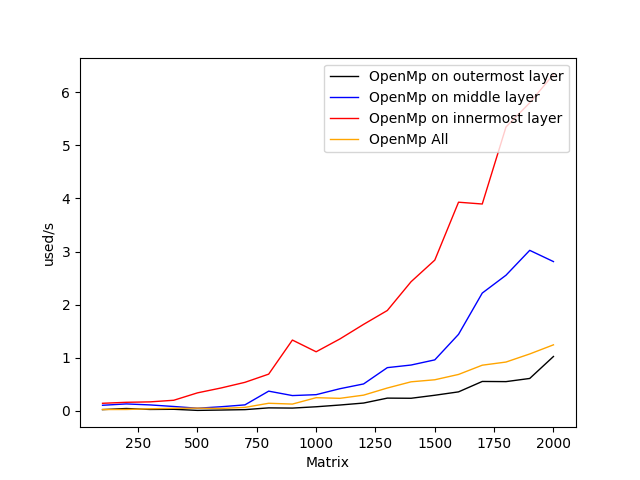
\includegraphics[scale=0.5]{3s}
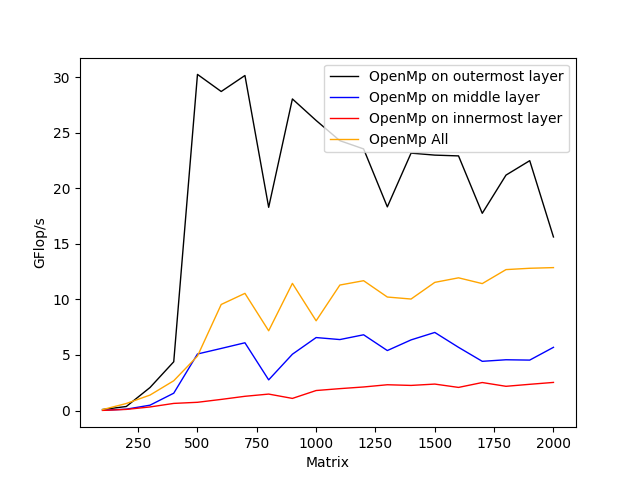
\includegraphics[scale=0.5]{3g}

\section{the parallel code of OpenBLAS}

GEMM (OpenBLAS)) used 0.00007 s, 27.03 GFlop/s

GEMM (OpenBLAS)) used 0.00022 s, 72.07 GFlop/s

GEMM (OpenBLAS)) used 0.00045 s, 119.21 GFlop/s

GEMM (OpenBLAS)) used 0.00100 s, 128.64 GFlop/s

GEMM (OpenBLAS)) used 0.00177 s, 140.92 GFlop/s

GEMM (OpenBLAS)) used 0.00307 s, 140.90 GFlop/s

GEMM (OpenBLAS)) used 0.00465 s, 147.56 GFlop/s

GEMM (OpenBLAS)) used 0.00662 s, 154.59 GFlop/s

GEMM (OpenBLAS)) used 0.00889 s, 163.99 GFlop/s

GEMM (OpenBLAS)) used 0.01230 s, 162.54 GFlop/s

GEMM (OpenBLAS)) used 0.01579 s, 168.59 GFlop/s

GEMM (OpenBLAS)) used 0.02032 s, 170.06 GFlop/s

GEMM (OpenBLAS)) used 0.02628 s, 167.17 GFlop/s

GEMM (OpenBLAS)) used 0.04007 s, 136.96 GFlop/s

GEMM (OpenBLAS)) used 0.03913 s, 172.50 GFlop/s

GEMM (OpenBLAS)) used 0.04913 s, 166.73 GFlop/s

GEMM (OpenBLAS)) used 0.05465 s, 179.79 GFlop/s

GEMM (OpenBLAS)) used 0.06469 s, 180.31 GFlop/s

GEMM (OpenBLAS)) used 0.07646 s, 179.42 GFlop/s

GEMM (OpenBLAS)) used 0.10112 s, 158.23 GFlop/s

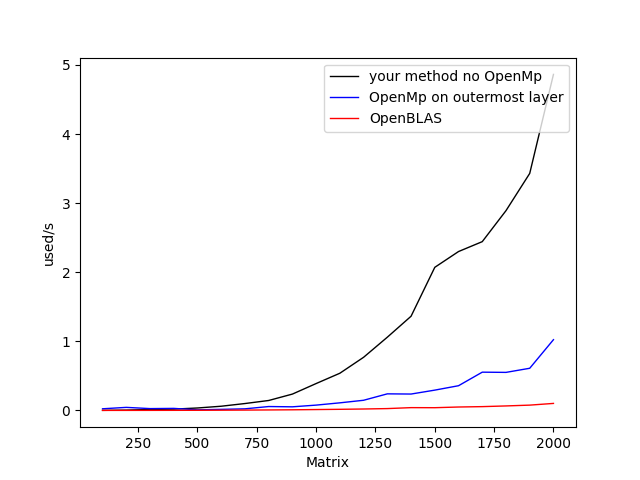
\includegraphics[scale=0.5]{4s}
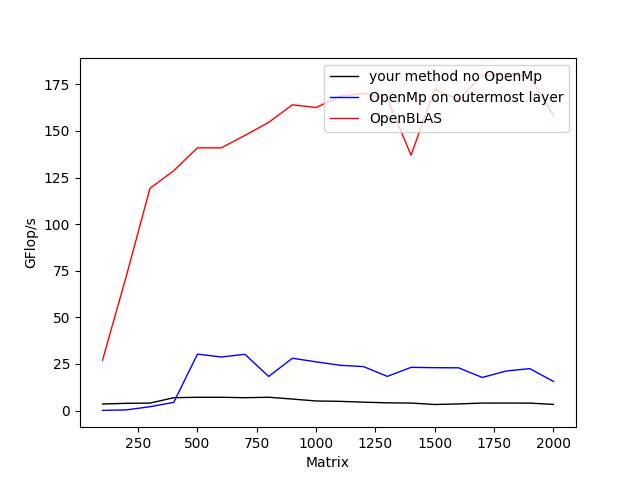
\includegraphics[scale=0.5]{4g}

\section{Original GEMM code optimized in any way}

I don't think of a better way for speeding up the matrix multiplication.
For the code, the only way I can optimized is the check results... As long as a number is fault, break from the loop.
But it seems meaningless if you need the sum of the wrong numbers.

\begin{lstlisting}
  int count2 = 0;
    for (int i = 0; i < m * n; i++)
        if (C_golden[i] != C_yours[i])
            count2++;
    if (count2 == 0)
        printf("GEMM (your method) PASS!\n\n");
    else
        printf("GEMM (your method) NOT PASS!\n\n");
\end{lstlisting}
   
to change:
\begin{lstlisting}
  int count2 = 0;
    for (int i = 0; i < m * n; i++)
        if (C_golden[i] != C_yours[i]){
            count2++;
            break
        }
    if (count2 == 0)
        printf("GEMM (your method) PASS!\n\n");
    else
        printf("GEMM (your method) NOT PASS!\n\n");
\end{lstlisting}
\begin{center}
\Huge{That's all!} \\
\Huge{End!} \\
\end{center} 
\end{document}
